\documentclass{article}
\usepackage{tabularx,fullpage,url}
\usepackage[top=1in, bottom=1in, left=.5in, right=.75in]{geometry}
\usepackage{amsmath,amssymb,graphicx,amsthm,xparse, color, mathrsfs} 
\usepackage{ epstopdf, fullpage}

\usepackage[ruled,vlined]{algorithm2e}
\usepackage{xifthen}
\usepackage{wrapfig}

\newcommand{\mypagebreak}{\begin{center}
		\noindent\makebox[\linewidth]{\rule{7.5in}{1pt}}
	\end{center}}
\bibliographystyle{siam}
\newcommand{\minimize}[1]{\underset{#1}{\text{minimize}}}
\newcommand{\maximize}[1]{\underset{#1}{\text{maximize}}}
\newcommand{\mini}[1]{\underset{#1}{\text{min}}}
\newcommand{\argmin}[1]{\underset{#1}{\text{argmin}}}
\newcommand{\st}{\text{subject to}}
\newcommand{\rank}{\textbf{rank}}
\newcommand{\epi}{\mathbf{epi}}

\newcommand{\diag}{\textbf{diag}}
\newcommand{\mb}{\mathbf}
\newcommand{\R}{\mathbb R}
\newcommand{\mle}{\mathbf{MLE}}
\newcommand{\map}{\mathbf{MAP}}
\newcommand{\bE}{\mathbb E}
\newcommand{\mL}{\mathcal L}
\newcommand{\mH}{\mathcal H}
\newcommand{\mB}{\mathcal B}
\newcommand{\mN}{\mathcal N}
\newcommand{\mD}{\mathcal D}
\newcommand{\mC}{\mathcal C}

\newcommand{\mS}{\mathcal S}
\newcommand{\tr}{\mathbf{tr}}
\newcommand{\mrm}{\mathrm}
\newcommand{\proj}{\mathbf{proj}}
\newcommand{\prox}{\mathbf{prox}}
\newcommand{\sign}{\mathbf{sign}}
\newcommand{\range}{\mathbf{range}}
\newcommand{\var}{\mathbf{var}}
\newcommand{\vnull}{\mathbf{null}}
\newcommand{\pr}{\mathbf{Pr}}
\newcommand{\find}{\mathbf{find}}
\newcommand{\argmax}[1]{\underset{#1}{\mathrm{argmax}}}
\newcommand{\subjto}{\mathrm{subject~to}}


\newcommand{\red}[1]{{\color{red}#1}}
\newcommand{\blue}[1]{{\color{blue}#1}}

\newcommand{\gray}[1]{\textcolor{lightgray}{#1}}



\newcommand{\idx}[1]{{\scriptsize [#1]}}

\newcommand{\showpoints}[1]{\textbf{(#1)}}


\begin{document}
{\Large\textbf{CSE 353: Homework 5 \hfill
Due Friday, Nov. 18}}


\mypagebreak



\begin{enumerate}

\item \emph{Machine learning fundamentals.} \showpoints{3 points, 1pt each} Discuss the dangers of overfitting by answering the following questions.

\begin{tabular}[t]{lll}
\begin{minipage}{.7\linewidth}
\begin{enumerate}

\item I have spent the past decade of my life collecting data for a specific task, and I have finally accrued 100 data points. I want to use all this data to train my model, thereby giving the best model. My best friend thinks it's a bad idea. Why is that?




\item ``Fine!" I say to my best friend. I will instead divide my dataset into two sets: a train and test set. I will train my model over the train set and only report the score over my test set. One caveat, this model is a little sensitive to how many iterations I run gradient descent during training: if I run it for too long or too short, the performance will degrade. So, I use my test set to determine the best number of iterations to run. My best friend scowls at me and scolds me again. Why is that? What is the appropriate way to partition my data, to give the most generalizable evaluation?





\item Today, many machine learning subfields use standardized datasets. These databases are divided into three sets: training, validation, and testing. We can assume that everyone is honest, and uses each set appropriately. Still, people are saying that there is a danger of overfitting, simply by using the same test base so many times. Discuss this: do you agree or disagree with this fear? Can you give an example of when this type of methodology can lead to bad real world effects? Be specific.



\end{enumerate}
\end{minipage}
&$\;$&
\begin{minipage}{.3\linewidth}
\centering
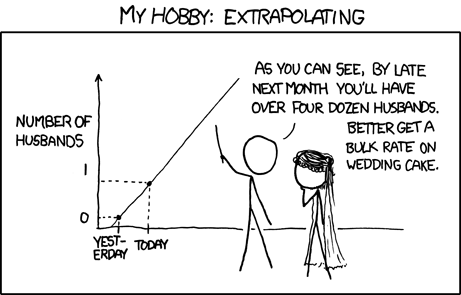
\includegraphics[width=\linewidth]{figs/extrapolating.png}\\(source: xkcd)
\end{minipage}
\end{tabular}




\item \textbf{Cross validation} \showpoints{4 pts}
\begin{itemize}
\item Download the dorothea dataset, and the corresponding ipython notebook (cross\_validation\_release.ipynb). Take a look at the dorothea pdf to understand the dataset and the task.

\item The Dorothea dataset is interesting and different from our previous datasets for 2 reasons. First, after loading the python notebook, run the cell that loads the data and take a look at some of the data qualities: namely, the number of features, labels, and sparsity of $X$. Additionally, write a script that returns some information on the balance of the training set labels. Write down some observations as to why this task might be different than previous binary classification tasks we've done in this class.



\item In the python notebook, I have given you a short implementation of a decision tree classifier using \texttt{scikit-learn}, with specifications 
\begin{center}\texttt{criterion='entropy',splitter='best',max\_depth=depth, class\_weight='balanced'}.
\end{center}
You are free to use this implementation, or whatever other implementation you'd like, as long as you preserve these parameters. (Keep the depth a variable, as we will change this throughout the exercise.)

Run this classifier over the training set, and evaluate the performance using \emph{misclassification rate} over both the test and train set. What do you observe? Did you do a good job? 






\item An alternative performance metric when dealing with unbalanced dataset is the F1 score, which can be written as 
\[
F1 = \frac{2PR}{P+R}, \qquad P = \frac{\text{\# detected }}{\text{\# retrieved}}, \qquad R = \frac{\text{\# detected }}{\text{\# relevant}}.
\]
For our data set, the event that $y_i = 1$ is a rare event, and we want to measure our ability to detect this rare event. So, an event is detected if $y_i = 1$ and $\hat y_i = 1$, retrieved if $\hat y_i = 1$, and relevant if $y_i = 1$.

Report the F1 score of the test and train set using the previously trained classifier. Does the F1 score look like a more reasonable performance metric for this task?








\item \emph{Without doing any cross validation}, sweep the depth of the tree through the values 2,3,...,10 and plot the train and test F1 scores for this sweep. Comment on what you see. 






\item Now, implement a K-fold cross validation, for $K = 5$. Take the train data, and partition it to $K$ segments. Over $i=1,...,K$ trials, take away the $i$th partition as a validation set, and record the F1 score over the sweep of tree depths over the remaining train set. Plot the F1 score over the \emph{validation set} for all $K$ trials. Comment on what you see. Is there a stable trend? 





\item Finally, plot the average validation F1 score against the test F1 score for the tree depth sweep. Does the best average F1 score of the validation set correspond, more or less, to a good F1 score  over the test set? Was this a successful venture? 




\end{itemize}



\item \showpoints{3 pts} \emph{Logistic regression for Binary MNIST} 
\begin{enumerate}
\item 
What is the gradient of the logistic loss function 
\[
f(\theta) = -\frac{1}{m}\sum_{i=1}^m \log(\sigma(y_ix_i^T\theta)), \quad \sigma(s) = \frac{1}{1+e^{-s}}
\]
where $y_i \in \{-1,1\}$? (Hint: Check out problem 1 again.)






\item \textbf{Coding gradient descent.}  Do \textbf{not} use  \texttt{scikit-learn} or other built in tools for this exercise. Please only use the packages that are already imported in the notebook. \footnote{This is to test your understanding of the basic machine learning concepts, like calculating accuracy and logistic loss; in the future you can use whatever tools you'd like.}

\begin{itemize}
\item Open \texttt{mnist\_logreg.ipynb}. We will use logistic regression to diffrentiate 4's from 9's, a notoriously tricky problem.
Run the first box to see what the data looks like.

\item In the second box I have set up the problem for you by pulling out the train and test set, selecting out only the data samples related to 4's and 9's. I have not altered the data in any other way. While other normalization tricks will help you improve the accuracy, for the purposes of this exercise we will forgo them, so that it's easy to compare everyone's solutions. 


 
\item Fill in the next box by providing code that will return the loss function value and the gradient. Make sure that everything is normalized, e.g. don't forget the $1/m$ term in the front of our loss function. Run the script.
If done correctly, you should see 
\begin{center}
\texttt{45.192, 12343.177}
\end{center}

\item Write a script that returns the classification accuracy given $\theta$. 
\item Use gradient descent to minimize the logistic loss for this classification problem. Use a step size of $10^{-6}$.

    \item \showpoints{1.5 pts} Run for 1500 iterations. In your report, give the plot of the train  loss and train/test misclassification rate, plotted as a function of \emph{iterations}. Report the final train and test accuracy values. 




\end{itemize}
 
\item \textbf{Coding stochastic gradient descent.} Do \textbf{not} use  \texttt{scikit-learn} or other built in tools for this exercise. Please only use the packages that are already imported in the notebook. Now, fill in the next box a function that takes in $\theta$ and a minibatch $\mathcal B$ as either a list of numbers or as an np.array, and returns the \emph{minibatch gradient}
\[
\nabla_\mB f(\theta) = \frac{1}{|\mB|}\sum_{i\in \mB} \nabla f_i(\theta)
\]
where $f_i(\theta)$ is the contribution to the gradient from datapoint $i$:
\[
f_i = -\log(\sigma(y_ix_i^T\theta)).
\]
Run the script. If done correctly, you should see the number 5803.5 printed out. 

\item \showpoints{1.5 pts} Write a script to run stochastic gradient descent over logistic regression. When coding up the minibatching, make sure you cycle through an entire training set once before moving on to the next epoch. Additionally, use \texttt{time()} to record the runtime, and compare the performance of gradient descent and stochastic gradient descent, using a minibatch size of 50 data samples and running for 50000 iterations. Return a plot that compares the objective loss, train accuracy, and test accuracy between the two optimization methods, as a function of \emph{runtime}. Comment on the pros and cons of the two methods.


\textbf{Important} Remember that calculating the loss function and train/test accuracy requires making \emph{full passes} through the data. If you do this at each iteration, you will not see any runtime benefit between stochastic gradient descent and gradient descent. Therefore I recommend you log these values every 10 iterations for gradient descent, and every 100 iterations for stochastic gradient descent. 




\end{enumerate}

\end{enumerate}


\end{document}